\chapter{Data exploration}
Here I describe the various data exploration techniques I have used. Lots of nice graphs. 


\section{A note about Test data, training data}

\section{Calculating common statistics}\label{sec:summary-statistics}
To start the data exploration, four common statistics, namely the mean, min, max and standard deviation, of every feature across the whole dataset was calculated. The standard deviation was calculated as (with $n$ equal the total number of rows in the dataset, and $x_i$ equal to the $i$'th value of any of the features)
\[
    s = \sqrt{\frac{\sum_{i=1}^n (x_i-\bar{x})^2}{n}}
\]
The source code for the calculations can be found in \appref{source-common-statistics} and all results in \appref{result-common-statistics}. Most results did not tell that much, but a few results stood out. These are shown in table~\ref{tbl:summary-stats-highlights}.
\begin{table}
    {\small\sffamily
        \begin{python}
            import scripts.commonstats_table as c; c.render('../sessions/9-data-exploration/src/summary_statistics.json', ['V5', 'V7', 'V9', 'E9', 'P8', 'P6', 'IsAlert'])
        \end{python}
    }
    \caption{Highlights from the results of the summary statistics. See~\appref{result-common-statistics} for all results.}
    \label{tbl:summary-stats-highlights}
\end{table}
The table shows that the features \fn{P8}, \fn{V7} and \fn{V9}, are zero throughout the whole dataset, and can be ignored. The features \fn{E9} and \fn {V5}, could be binary, but that is only speculation at the moment. Finally the feature \fn{P6} has a mean of 843.73 and a standard deviation of 2795.32, but its maximum is 228812.00, which is many, many standard deviations away from the mean. This could be a sign of some serious outliers, but it could as well be a single trial with a mean far from the other trials. Further investigation are needed to conclude anything here. Finally it is seen that the mean of the \fn{IsAlert} feature is only a little above 0.5, and therefore only a little over 50\% of the time are the drivers alert. This may be a bit surprising. \par
The results of this first step have been to exclude a few features, and get some rough ideas about the shape of some other features. It is now time to resally get to know the different features.

\section{Determining the datatype of features}
Since Ford would not disclose any information about the different features, it is important to get a good picture of which features are discrete/categorical and which features are continous. A natural first step to learn the datatype of the features, is to calculate the number of unique values each feature takes.
\subsection{Unique values}\label{sec:unique-values}
It requires a little thought to pinpoint exactly what needs to be calculated. On one hand it is natural to calculate the number of unique values a feature takes across the whole dataset. On the other hand it could happen, that a discrete feature might have only (eg.) 3 unique value within any trial, but the values differ between various trials. This way we would have a feature with 1500 unique values across the whole dataset, but with max 3 unique values within any given trial. Therefore the number of unique values within a trial are calculated for every feature and every trial. Based on this result, the minimum and maximum number of unique values within a single trial, is calculated for every feature. The source code can be found in \appref{source-unique-values} and results are shown in table~\ref{tbl:result-unique-values}.\mytodo{The result table in appendix or in report?} \par
\begin{table}
    {\small\sffamily
        \begin{python}
            import scripts.uniquevalues_table as c; c.render(['V7','V9','P8'])
        \end{python}
    }
    \caption{The minimum and maximum number of unique values within the trials, for every feature in the dataset. Also the total number of unique values for each feature, across the whole dataset, are shown.}
    \label{tbl:result-unique-values}
\end{table}
A couple of things should be noticed about the results. Almost all features have som trials where they only take on one unique value. For categorical features, this could be perfectly normal, but for a continous feature it seems to be pretty unlikely to have only one value in a trial spanning two minutes. Is a feature, that in some trials seems continous, but then only have one value in other trials, just turned off in the latter trials? And how should the feature be handled in trials where it is ``off"?. This discussion is continued in section~\ref{sec:outlier-detection} about outlier detection. \par

From table~\ref{tbl:result-unique-values} it is also seen, that only features \fn{P1}, \fn{P2} and \fn{V11} is consistently having lots of unique value, across all trials. It seems fair to call these features continous. Feature \fn{V1} have some trials where it takes on 969 different values, but it also have trials with only one unique value. Across the whole dataset it takes on 12374 unique values. This could be explained by feature \fn{V1} being continous in a small number of trials (about 15-30), and turned ``off" in all other trials. Further exploration will show whether it is true or not. \par

Another interesting detail is that there are two pairs of features ((\fn{P3},\fn{P4}), (\fn{P6},\fn{P7})) in the results, that share exactly the same number of unique features. Both min and max and total. This indicates a possible relationship between the features, and later (section~\ref{sec:scatterplots}) it is shown that this is in fact true. \par

A final remark about the number of unique values, is that feature \fn{E9} and \fn{V5} indeed are binary. Also if a limit of max 40 unique values within a single trial is set, as an indicator for categorical features, \fn{E3}, \fn{E7}, \fn{E8}, \fn{V3} and \fn{V10} are seen to be categorical. \par

\subsection{Plotting some features}\label{sec:plotting-features}
To get a more nuanced picture of the various features, it is now time to visualize the data. The first thing of interest is to plot every feature for a couple of trials, to see the structure of the features, and how much they vary between different trials. For a start some random plotting was done in the interactive ipython-shell\footnote{For details about the software setup used, see chapter~\ref{chp:tools}}. \par
\begin{figure}[!hbtp]
    \centering
        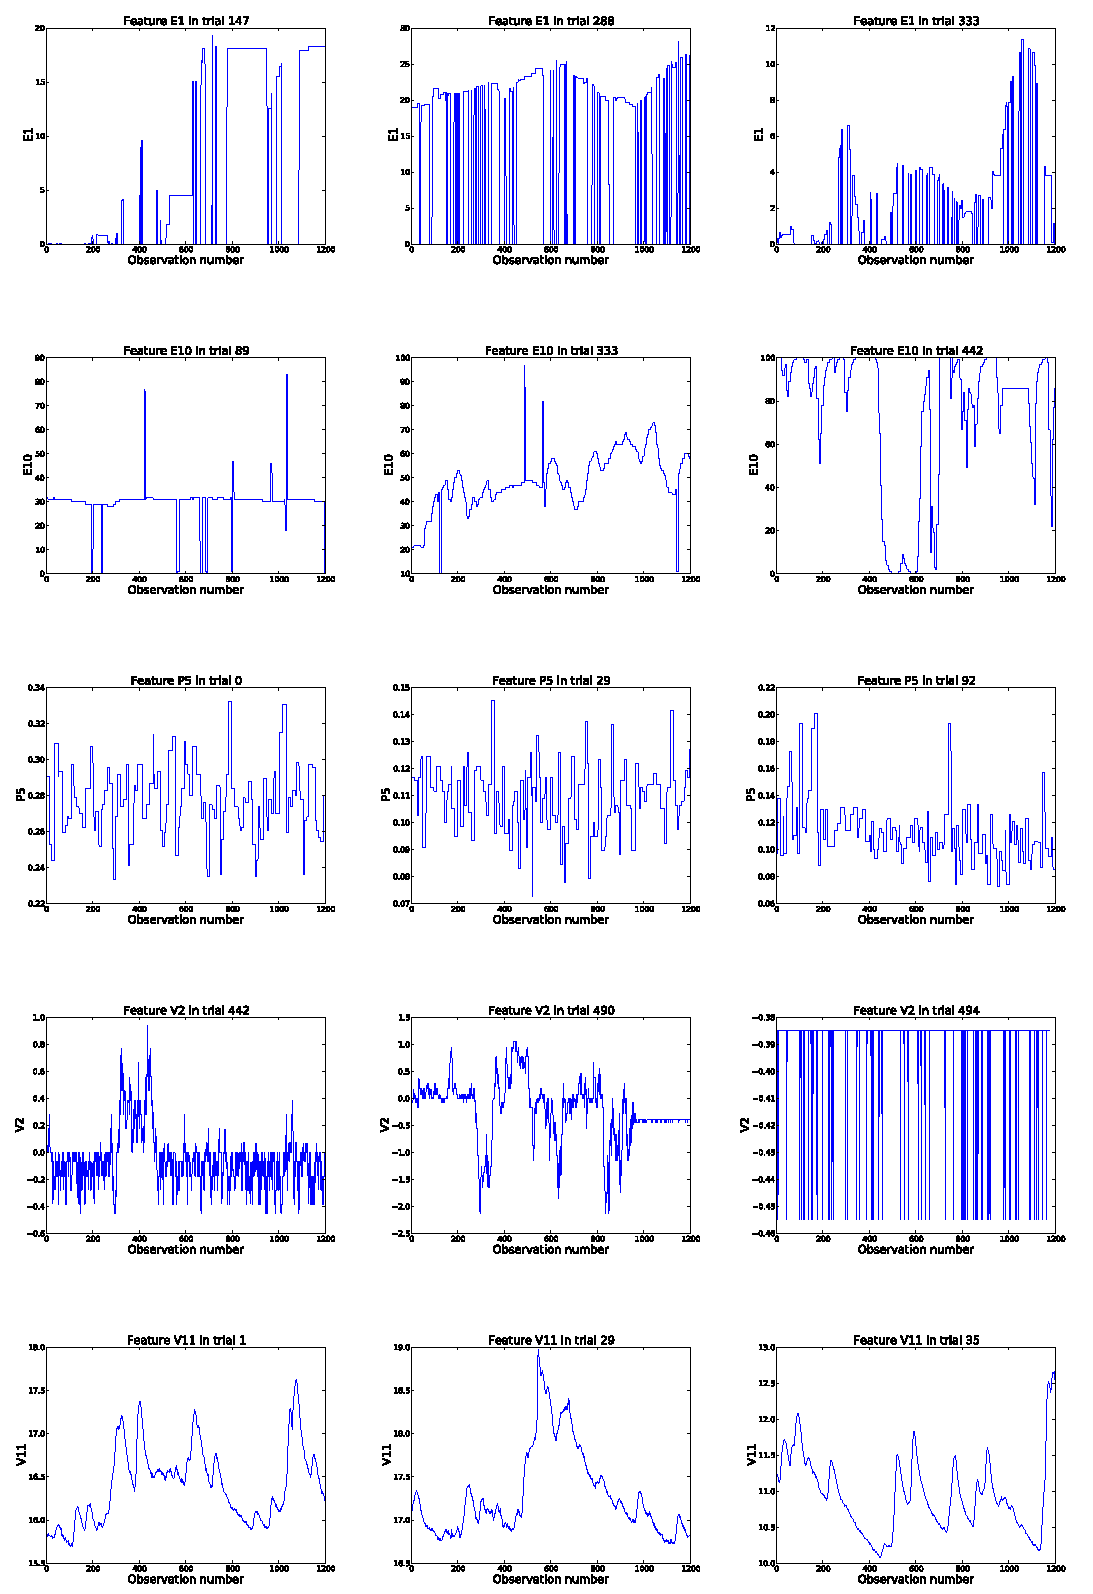
\includegraphics[width=\textwidth]{media/feature-plots-sheet.pdf}
    \caption{Plots of the features \fn{E1}, \fn{E10}, \fn{P5}, \fn{V2}, \fn{V11}, for a couple of trials. The trials was selected to show the diversity a single feature exhibits between trials.}
    \label{fig:exploratory-feature-plots}
\end{figure}
Some selected plots from the interactive plotting session are shown i figure~\ref{fig:exploratory-feature-plots}. The main results from the introductory plotting of features are that: 
\begin{itemize}
    \item A feature varies alot in structure between different trials
    \item Many features are constant in some trials (was already hinted at in section~\ref{sec:unique-values})
    \item Some features deviates a lot from their ``normal" structure, in a few trials (more about that in section~\ref{sec:outlier-detection} about outliers).
    \item The feature \fn{P2} looks like pure noise\mytodo{Is this right?}
    \item The features \fn{E3}, \fn{E7}, \fn{E8}, \fn{V3} and \fn{V10} does indeed seems to be categorical features, although \fn{V3} do have some extra structure\mytodo{What do I mean? Plot categorical features?}
\end{itemize}
Apart from the observations above, a subjective conclusion from the plots of the features is that the data quality could be better. Since the data quality isn't perfect it is important to consider how outliers should be dealt with. This i what the next section is about.


\section{Outlier detection}\label{sec:outlier-detection}
The textbook approach for detecting outliers is to create boxplots of the different features, and then argue that data points outside the 95-percentile should be removed. Although this is a naive approach some useful information could be obtained from boxplots of the features. But i doesn't necessarily make sense to make boxplots of the features for the whole dataset. Some features have the same structure in different trials, but their mean varies. Eg. feature \fn{V11} in trials 29 and 35 have similar structure but the range in trial 29 is $[16.75, 19]$ and $[10,12.6]$ in trial 35 (see figure~\ref{fig:exploratory-feature-plots}). If a feature has a different mean in only a few trials, those datapoints could be seen as outliers, if we look at the feature across the whole dataset. Instead boxplots of the features for the 50 first trials are created. This also gives a visual idea about how feature means varies from trial to trial. 
\subsection{Making boxplots of features}
The boxplots for 4 selected features are shown i figure~\ref{fig:boxplots}. All boxplots are in \appref{result-boxplots}, and the source code can be seen in \appref{source-boxplots}. \par
\begin{figure}
    \begin{tabularx}{\textwidth}{ X X }
        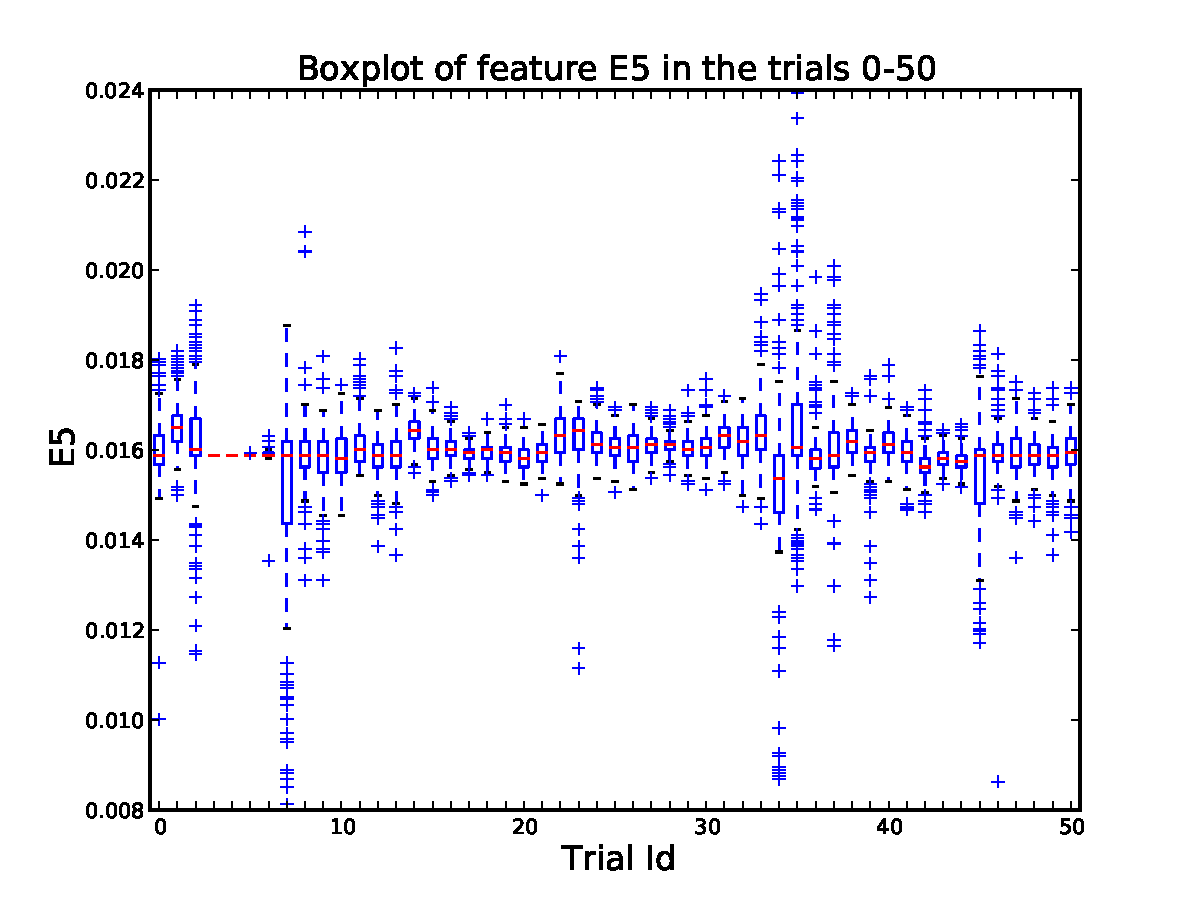
\includegraphics[width=.5\textwidth]{../sessions/11-boxplots-scatterplots/plots/boxplots/E5-t0-t50.pdf} &
         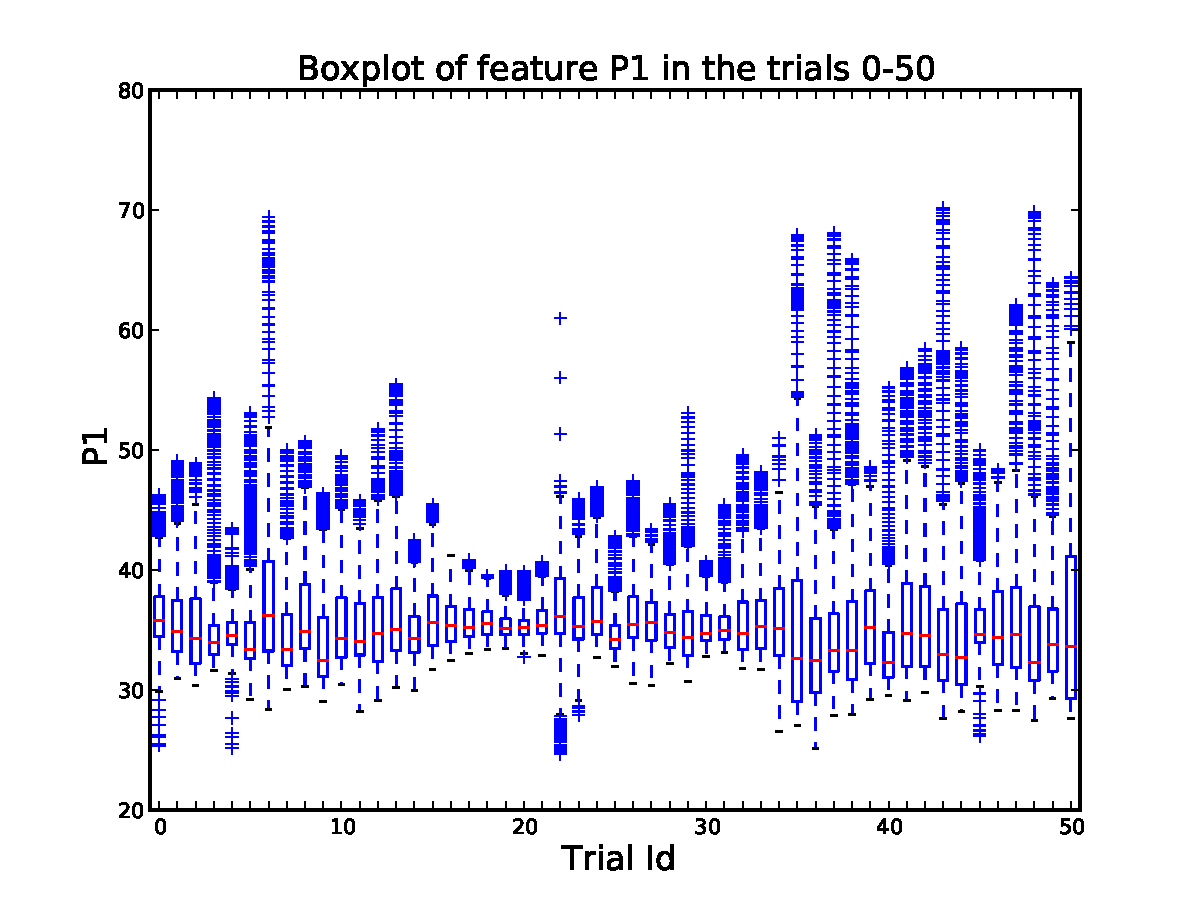
\includegraphics[width=.5\textwidth]{../sessions/11-boxplots-scatterplots/plots/boxplots/P1-t0-t50.pdf}\\
        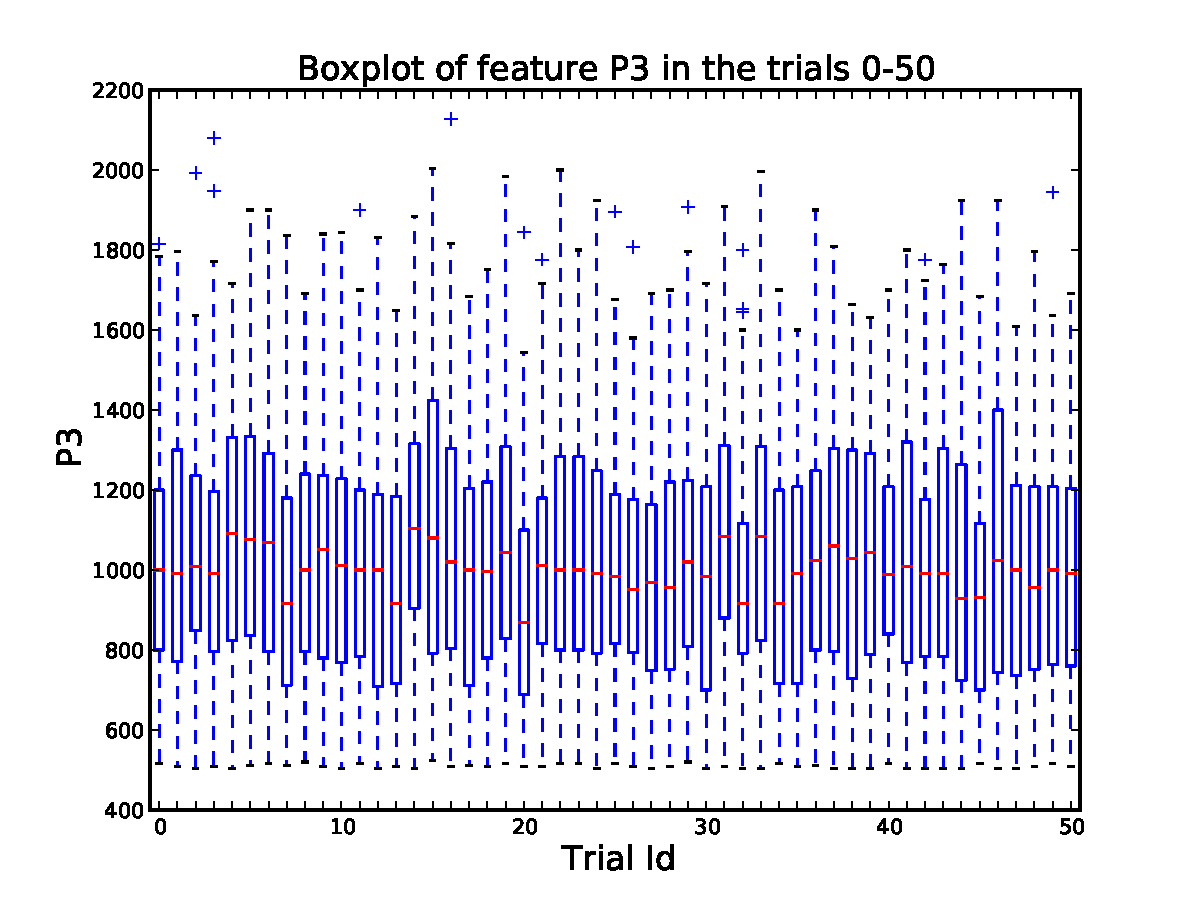
\includegraphics[width=.5\textwidth]{../sessions/11-boxplots-scatterplots/plots/boxplots/P3-t0-t50.pdf} &
         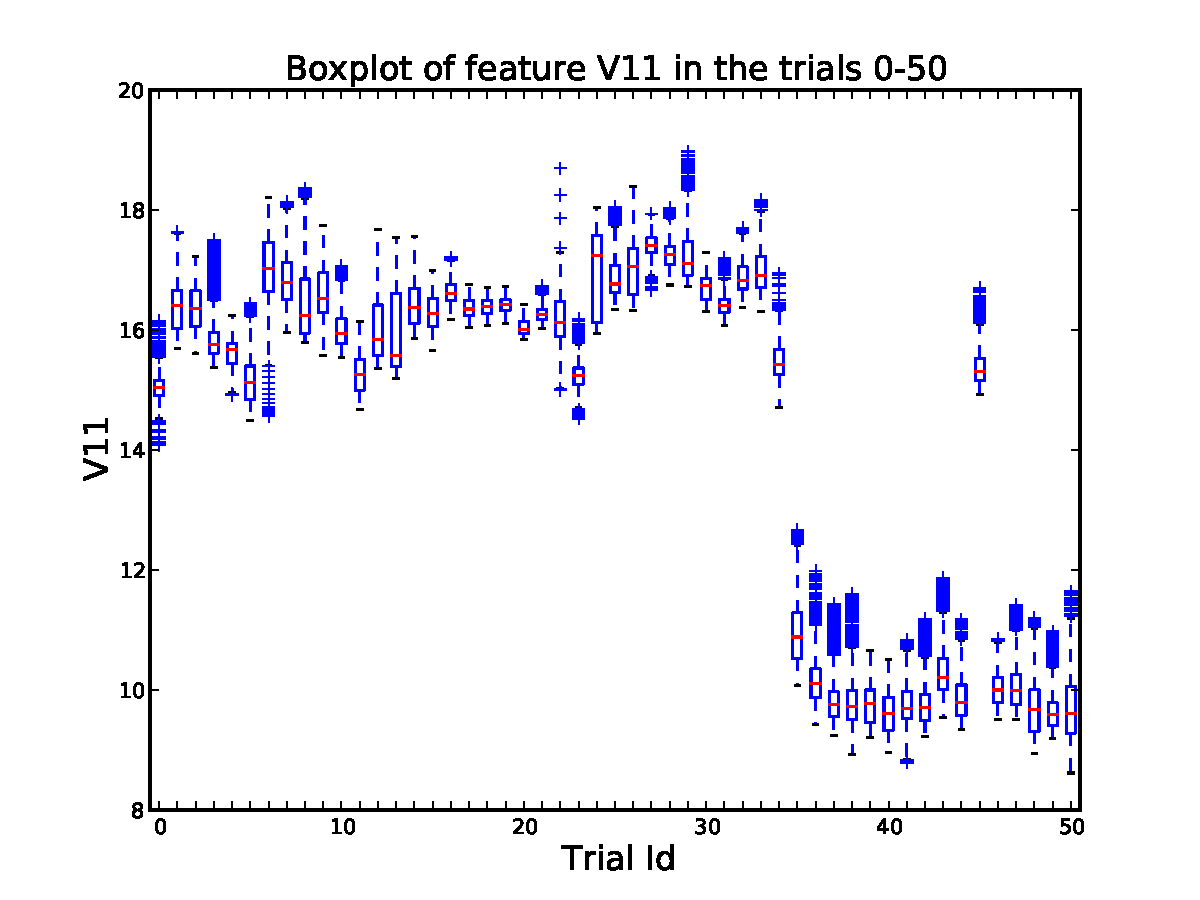
\includegraphics[width=.5\textwidth]{../sessions/11-boxplots-scatterplots/plots/boxplots/V11-t0-t50.pdf}
    \end{tabularx}
    \caption{Boxplots of feature \fn{E5}, \fn{P1}, \fn{P3} and \fn{V11} in the first 50 trials}
    \label{fig:boxplots}
\end{figure}
From the boxplots a couple of things are of interest.
\begin{itemize}
    \item For some features the trial mean varies a lot between different trials \mytodo{Remember to check with boxpots in appendix}
    \item Within a single trial some features still have a lot of data points outside the 95 percentile. See eg. \fn{P1} in figure~\ref{fig:boxplots} \mytodo{Check the right name (percentile?)}
\end{itemize}
As many features have datapoints outside the 95 percentile even within a single trial, the next step could be to categorize these datapoints as outliers. But inspection of some examples of specific features in specific trials, shows that it would be wrong to remove these ``outliers". Eg. feature \fn{V11} in trial 29 is plotted in figure~\ref{fig:exploratory-feature-plots} and seems to be perfectly normal. Careful inspection of the boxplot for feature \fn{V11} in trial 29 (figure~\ref{fig:boxplots}) shows that the feature has many outliers in this specific trial. \par
The boxplots do not correctly identify the outliers in the dataset, and another method is therefore neede.

\subsection{Making layered feature plots}
Instead of trying to categorize single datapoints as outliers, it may make more sense to define a specific feature in a specific trial as an outlier. The fact that some features deviates a lot from their normal structure, in a few trials was already mentioned in section~\ref{sec:plotting-features} about exploratory plotting of features. Since the exploratory plotting was a rather unstructered process, a more thorough picture, of the structure of the different features across all trials, is needed. One way to get a better picture is by plotting all trials of a single feature, in a single plot. The graph of each trial is given a low opacity and then all 500 trials\mytodo{update number based on number of training trials} are plotted on top of each other. That way the common structure of a feature across trials are visualized, and possible outlier trials can be detected. Two examples of this plot type can be seen in figure~\ref{fig:layered-feature-plots}\footnote{Source code for the layered feature plots can be found in \appref{source-layered-feature-plots} and the results are in \appref{result-layered-feature-plots}} \par
\begin{figure}
    \centering
    \subfloat[]{\includegraphics[width=.5\textwidth]{../sessions/22-create-transparent-feature-plots/plots/naive_p6.png}\label{fig:layered-all-trials}}
    \subfloat[]{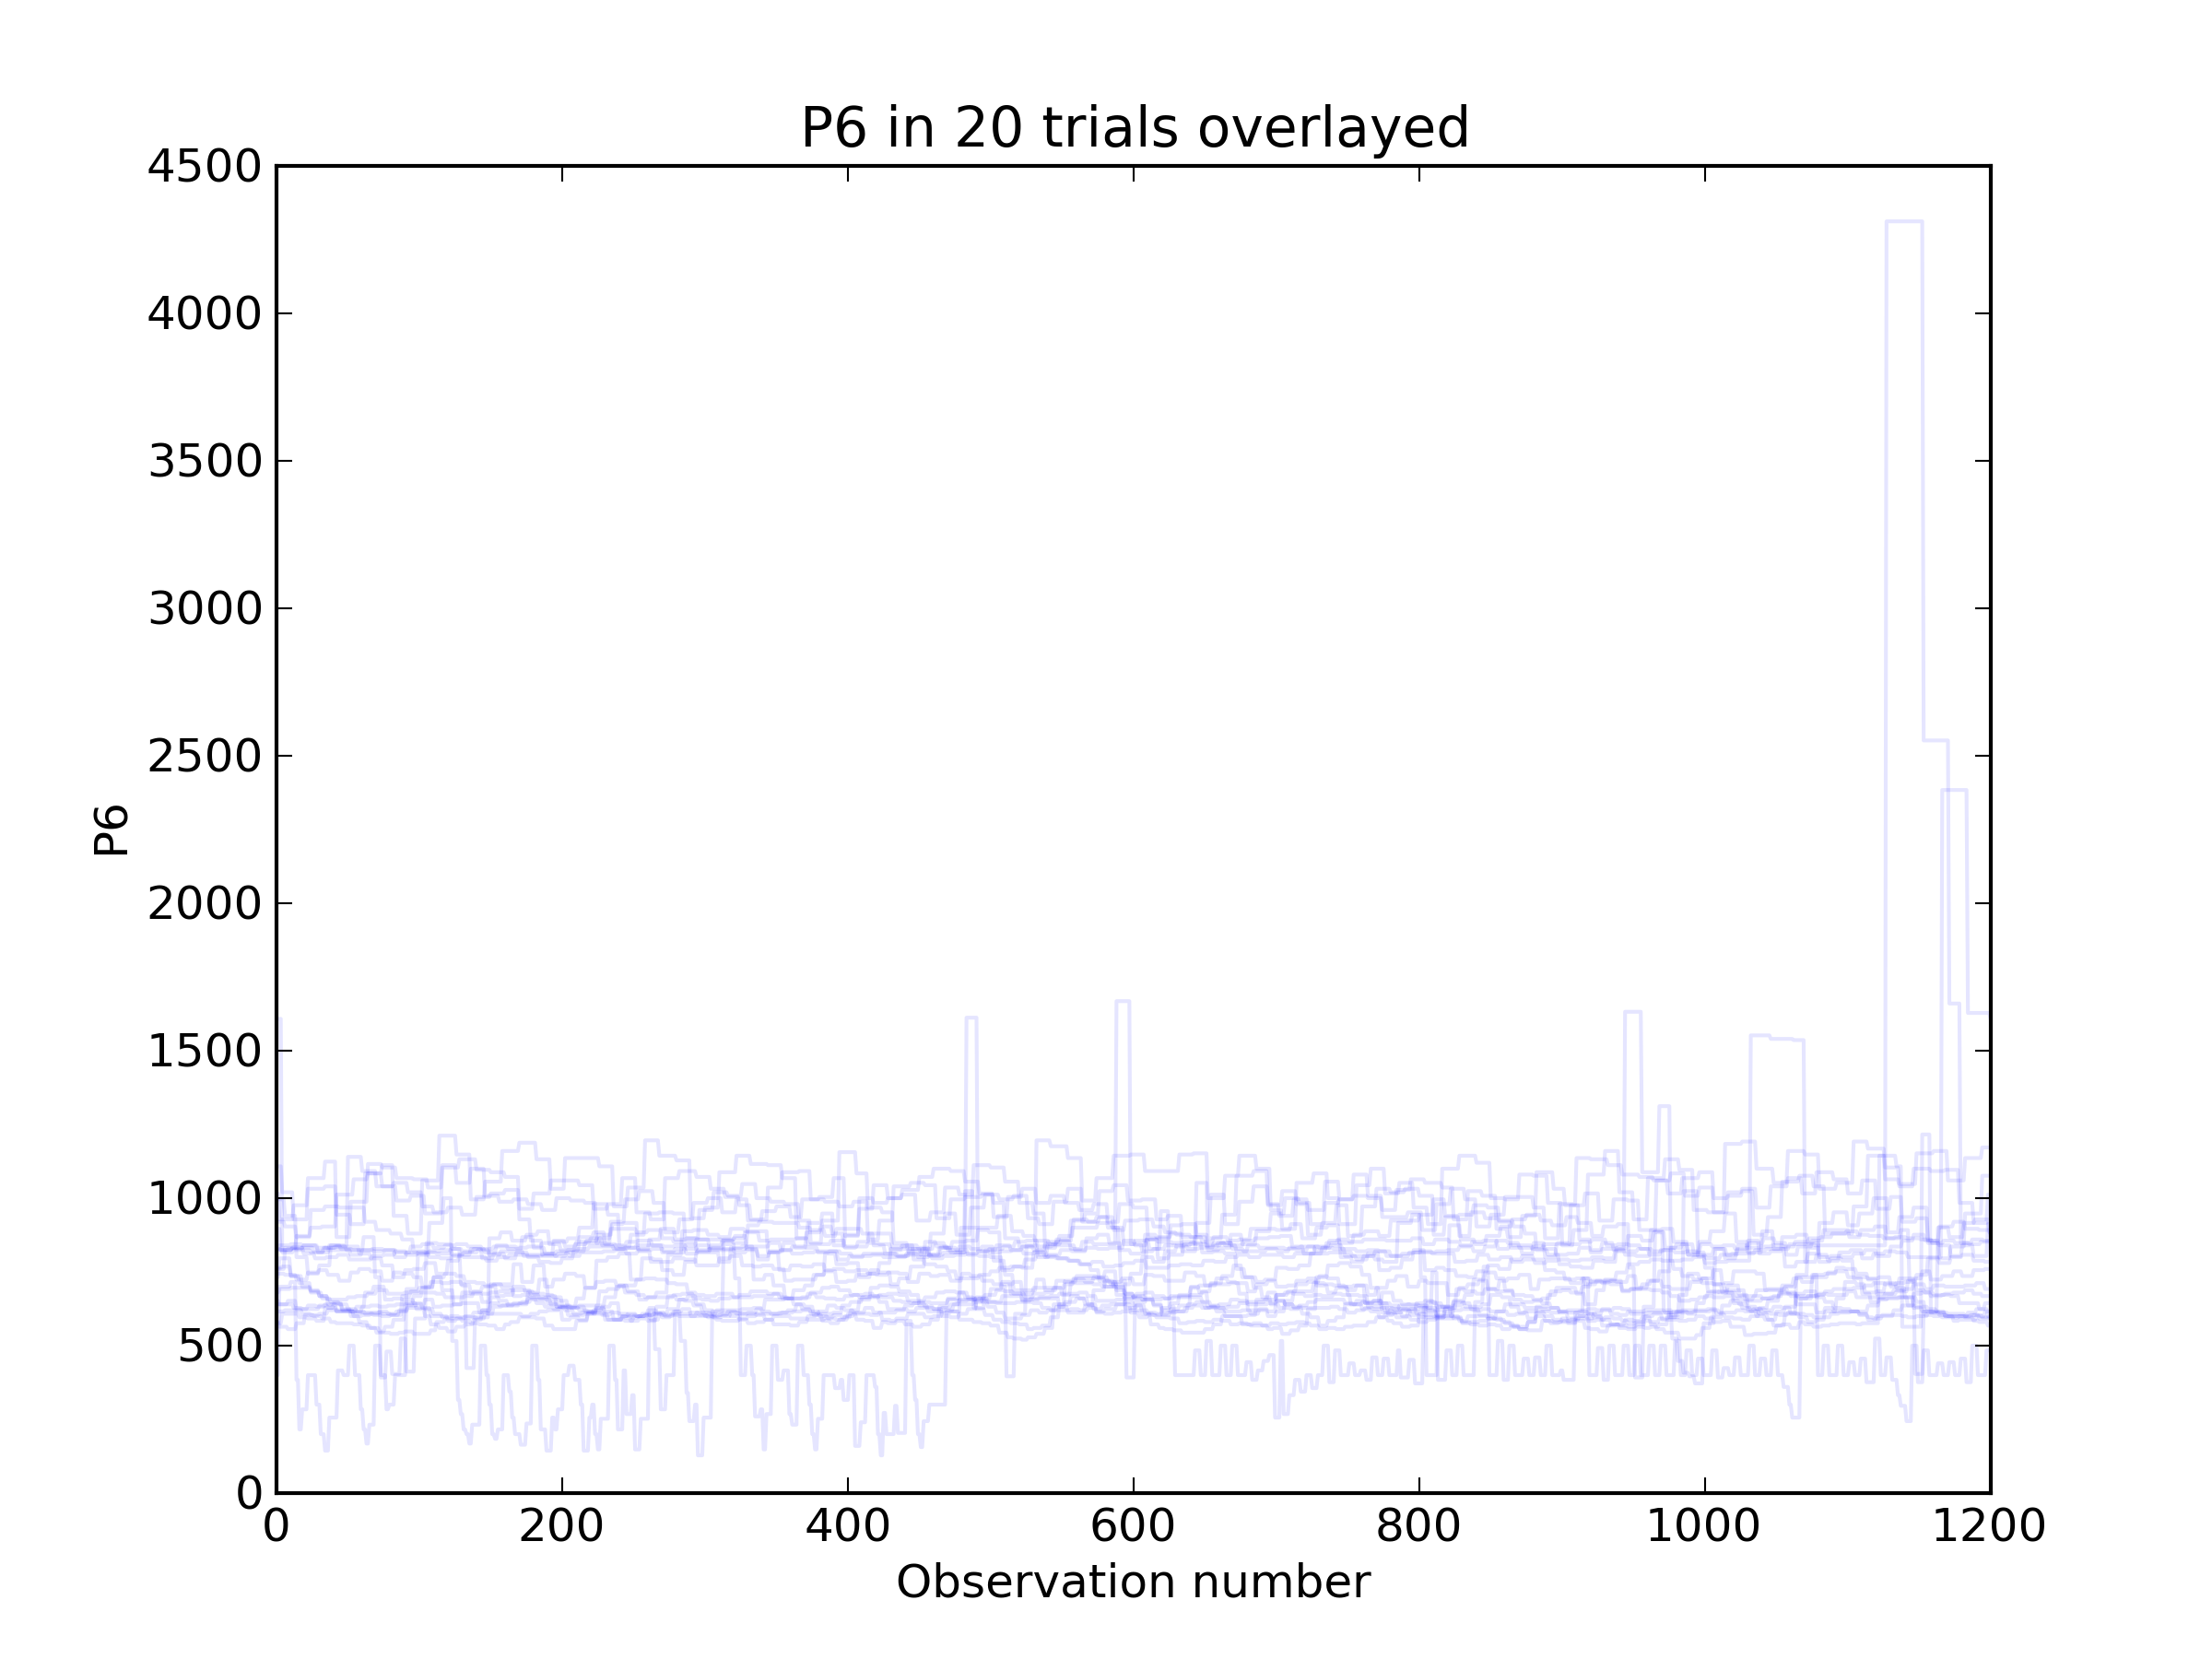
\includegraphics[width=.5\textwidth]{../sessions/22-create-transparent-feature-plots/plots/P6_20-trials.png}\label{fig:layered-20-trials}}
    \caption{Layered feature plots of feature \fn{P6}. All 500 trials are shown on the left. A couple of possible outliers are seen. On the right only 20 randomly chosen trials are plotted}
    \label{fig:layered-feature-plots}
\end{figure}
From the layered feature plots it is confirmed that many features have some trials that seems to deviate from the normal pattern of the feature. Using feature \fn{P6} as an example, it is seen in figure~\ref{fig:layered-all-trials} that \fn{P6} in almost all trials lies within the range $[0,2000]$. But one trial have a max value larger than 200000. This behaviour was hinted in section~\ref{sec:summary-statistics} and now there is a visual confirmation. \par
The question is, how should this ``outlier" trial of feature \fn{P6} be handled? One approach is to exclude the trial from the dataset. But as nothing about the origin of the dataset is known, it can't be justified with a commen sense argument, and if this trial is excluded then how is the line between outlier and normal drawn? There is a couple of other trials where the \fn{P6} feature has values as high as 20000, but should this be seen as outliers? And are there other ways a trial could be an outlier than the scale? In figure~\ref{fig:layered-20-trials} most trials have the same structure, but the trial with the lowest mean has a noticeable different shape than the other trials. It somehow has a baseline at the value 400 and then oscillates a a higher frequency than the other trials. Is this an outlier? If it is regarded as an outlier many other trials could possibly be classified as outliers, and we're are still only looking at one feature. If the same amount of cleaning is done for the other features, not much is left for the ``normal" dataset. \par

The immediate conclusion is that the outlier detection easily becomes, either too all-encompassing or is done in an inconsistent manner. An alternative way to tackle the trials with datapoints with large values, could be to do some kind of variable transformation (eg. taking the log) of the feature. This could be a solution and the idea is investigated a little more in section~\ref{sec:recreating}.

\subsection{Features that are constant in a trial}
Another type of potential outlier trials, are all the trials where one or more features are constant throughout the trial. This could be a sign of a failure in the measurement equipment, and then maybe the trial should be regarded as an outlier? A great example is the \fn{IsAlert} feature, that is the feature that should be predicted by the classifier. In 142 out of the 400 trials the \fn{IsAlert} feature is constant and in 127 of the trials with a constant value, the driver isn't alert. At first it may seem a bit odd, and indeed some of the contestants of The Ford Challenge revealed that they had excluded all trials where the \fn{IsAlert} feature was 0 throughout the trial (see \citet{kaggle_forum_328_reply_2}). But it is speculative to do, since the precise meaning of the \fn{IsAlert} feature isn't known, let alone the fact that, measurering human alertness with a binary variable is speculative by itself. \par
As it seems to speculative to exclude features with constant values, this idea won't be pursued any further. Instead the focus changes from "finding features to get rid of" till "finding features that could be benificial for classification" as the next section is all about finding features that can discriminate between alert/not-alert drivers.


\section{Finding possible discriminating features}
In this section all features are examined in an attempt to find one or more features that are in some way correlated with the \fn{IsAlert} feature that should be predicted. 

\subsection{Testing binary features}
A tempting first attempt at finding a feature that can be used to predict the \fn{IsAlert} feature, is to look at the two binary features \fn{V5} and \fn{E9} and see if they are correlated with the predictor\mytodo{What is the \fn{IsAlert} feature called?}.

\subsection{Scatterplots}\label{sec:scatterplots}
A great way to visualize whether a pair of features can be used to discriminate between datapoints where the driver is alert and where he/she is not alert, is to create scatterplots of the possible pair of features. Since feature \fn{V7}, \fn{V9} and \fn{P8} are removed and feature \fn{E3}, \fn{E7}, \fn{E8}, \fn{E9}, \fn{V3}, \fn{V5} and \fn{V10} was found to be categorical, only 20 features are left for the scatterplots. Since the order of the two features in a scatterplot doesn't matter there is a total of 
\[
    \begin{pmatrix}
        20 \\
        2
    \end{pmatrix} = 190\:\text{combinations}
\]
All combinations of the 20 features was plotted\footnote{Source code can be found in \appref{source-scatterplots} and the results in \appref{result-scatterplots}}, and no interesting results was found; at least not regarding feature pairs that could classify the \fn{IsAlert} feature. One interesting result was found though. As can be seen in figure~\ref{fig:scatterplots}
\begin{figure}
    \begin{tabularx}{\textwidth}{ X X }
        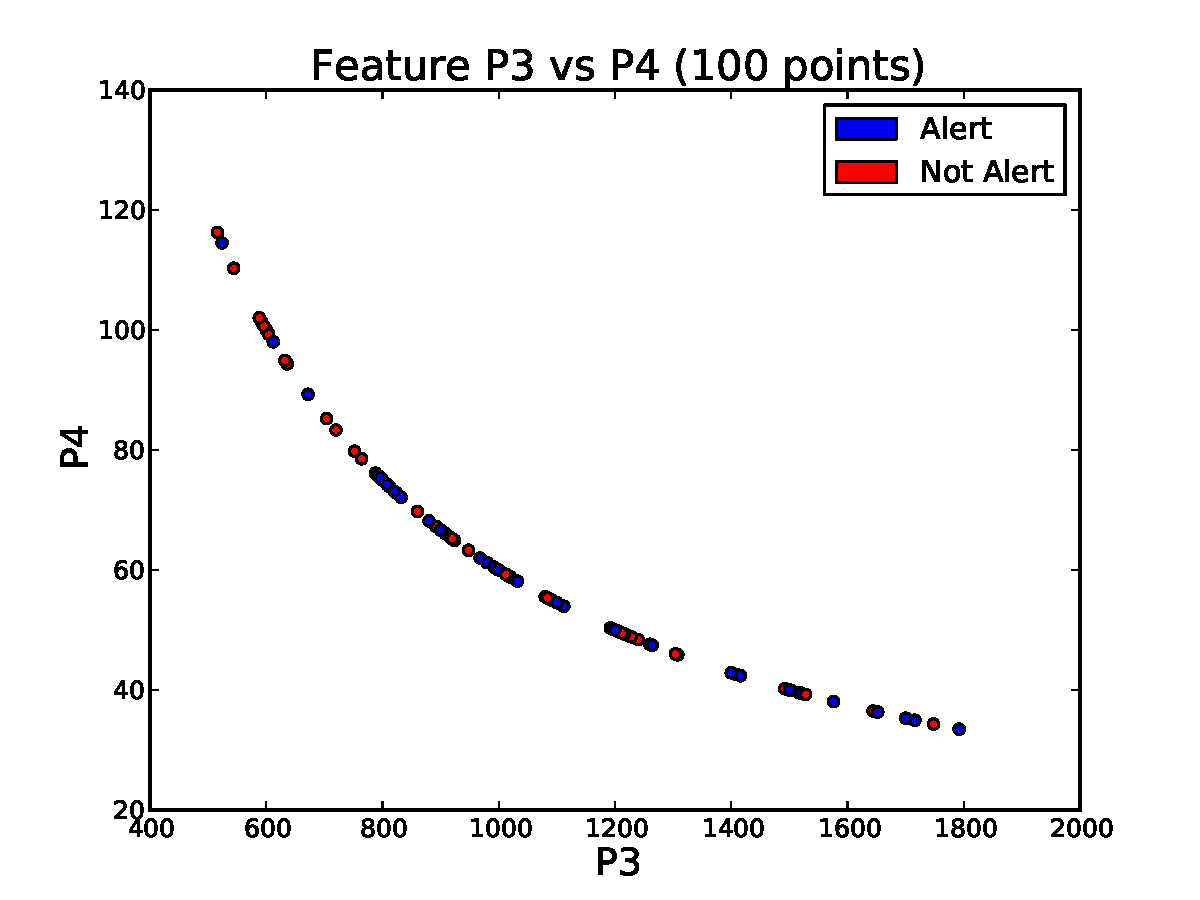
\includegraphics[width=.5\textwidth]{../sessions/24-writing-helper-scripts/plots/scatterplots/P3-P4.pdf} &
        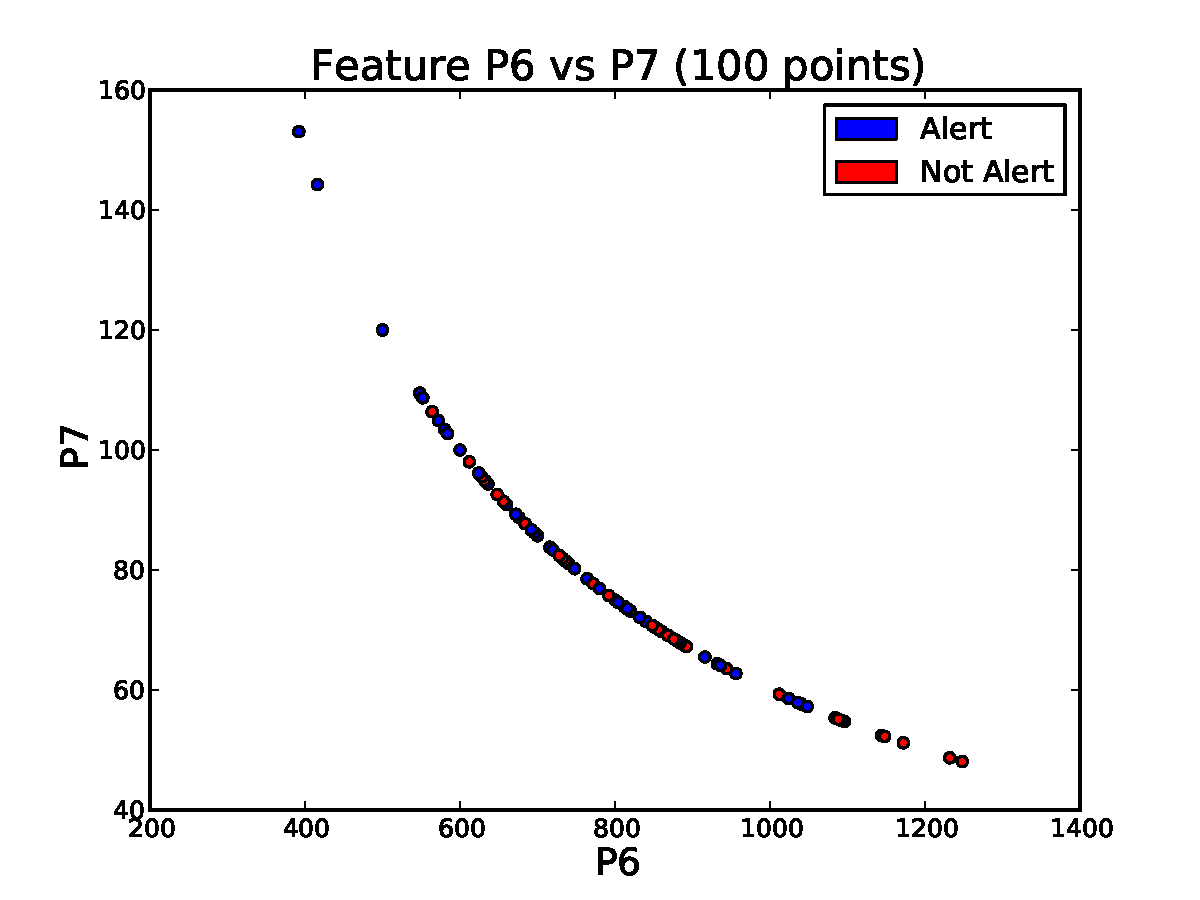
\includegraphics[width=.5\textwidth]{../sessions/24-writing-helper-scripts/plots/scatterplots/P6-P7.pdf}
    \end{tabularx}
    \caption{Scatterplots of the feature pairs (\fn{P3}, \fn{P4}) and (\fn{P6}, \fn{P7}). An arithmetic relationship between the features is clearly present}
\end{figure}


\section{Principal Component Analysis}
\subsection{Theory}
The idea in Principal Component Analysis (PCA) is to find a mapping from a $d$-dimensional input space, to a new $k$-dimensional space (with $k<d$), while keeping as much of the variation in the input data, as possible. To begin with let $k=1$. Then the subspace is identified by a $d$-dimensional vector $\ve{w}_1$, that without loss of generality is assumed to have length $\norm{\ve{w}_1}=1$. \par
For any vector $\ve{x}$ in the input space, the projection onto $\ve{w}_1$ is given by
\[
    z_1 = \ve{w}_1^T \ve{x}
\]
and we now wish to maximize the variance of $z_1$. By the definition of variance we get (with $\ve{\mu}=\expop{\ve{x}}$)
\begin{align*}
    \varop{z_1} &= \varop{\ve{w}_1^T\ve{x}} \\
    &= \expop{(\ve{w}_1^T\ve{x} - \ve{w}_1^T\ve{\mu})^2} \\
    &= \expop{(\ve{w}_1^T\ve{x} - \ve{w}_1^T\ve{\mu})(\ve{w}_1^T\ve{x} - \ve{w}_1^T\ve{\mu})} \\
    &= \expop{\ve{w}_1^T(\ve{x}-\ve{\mu})(\ve{x}-\ve{\mu})^T\ve{w}_1} \\
    &= \ve{w}_1^T\expop{(\ve{x}-\ve{\mu})(\ve{x}-\ve{\mu})^T}\ve{w}_1 \\
    &= \ve{w}_1^T\ve{\Sigma}\ve{w}_1
\end{align*}
where $\ve{\Sigma} = \covop{\ve{x}}$. So to maximize the variance of $z_1$ is the same as maximizing $\ve{w}_1^T\ve{\Sigma}\ve{w}_1$, subject to the contraint that $\ve{w}_1^T\ve{w}_1=1$. By introducing a Lagrange multiplier $\alpha$, we get
\[
    \max_{\ve{w}_1} \ve{w}_1^T\ve{\Sigma}\ve{w}_1 - \alpha(\ve{w}_1^T\ve{w}_1 - 1)
\]
This is a normal, unconstrained maximization problem. Taking the derivative with respect to $\ve{w}_1$, and setting this equal to 0, gives
\begin{align*}
    2\ve{\Sigma}\ve{w}_1 - 2\alpha\ve{w}_1 &= 0 \myimp \\
    \ve{\Sigma}\ve{w}_1 &= \alpha\ve{w}_1
\end{align*}
which is true exactly when $\ve{w}_1$ is an eigenvector of $\ve{\Sigma}$ and $\alpha$ is the corresponding eigenvalue.
Giver det mening på binære variable?

\section{Conclusions}

